%%%%%%%%%%%%%%%%%%%%%%%%%%%%%%%%%%%%%%%%%%%%%%%%%%%%%%%%%%
%   Autoren des Abschnitts:
%   Jakob Kautz
%   Olivier Stenzel
%%%%%%%%%%%%%%%%%%%%%%%%%%%%%%%%%%%%%%%%%%%%%%%%%%%%%%%%%%

% !TEX root =  master.tex
\chapter{Umsetzung - Hardware} \label{umsetzungHW}
\chapterauthor{Jakob Kautz, Olivier Stenzel}

\nocite{*}
- Probleme, Schwierigkeiten, Änderungen während der Umsetzung

Nachdem die Planungsphase abgeschlossen war, mussten die Überlegungen umgesetzt werden.
Im Rahmen dieser Arbeit wurde ein Prototyp gebaut, welcher 8 Tasten anspielen kann.
Zusätzlich wurde die Elektronik mit LEDs so erweitert, dass man das Drücken von 40 Tasten simulieren kann. % @Note(Val): Entweder hier oder an späterer Stelle erwähnen, dass es an sich trivial aber halt zeitaufwendig wäre, mehr Tasten anspielbar zu machen
% @Note(Val): Ich würde hier vielleicht noch gar nicht erwähnen, dass nur 8 Tasten anspielbar sind, weil die ganze Umsetzung ja mit dem Ziel 88 Tasten anspielbar zu machen lief. Kostenschätzung, etc. sind deshalb ja auch höher. Vielleicht ist es besser hier zu sagen, dass das Ziel war, den Prototypen mit möglichst vielen spielbaren Tasten zu gestalten, aber nur 8 bis dato erledigt wurden

\section{Materialien}
\chapterauthor{Jakob Kautz}
\subsection{Liste der Bauteile}
%TODO(Jay): Fix List
\begin{table}[htbp]
    \centering
    \begin{tabular}{|m{3.8cm}|m{1.7cm}|m{8cm}|}
        \hline
        \textbf{Bauteil} &  \textbf{Anzahl} & \textbf{Begründung}  \\
        \hline
        Hubmagnete & 88 & jede Taste braucht einen Hubmagneten um angespielt zu werden \\ % @Note(Val): Erwähnen, dass nur 8 der Hubmagnete benötigt wurden
        \hline
        Stromversorgung & 1 & Externe Stromversorgung für die Aktuatoren, da diese mehr als die 5V Vcc des Arduinos brauchen \\
        \hline
        Arduino & 1 & Kommunikation \\
        \hline
        Breadboard & 2 & Kleinstromschaltung \\
        \hline
        Schaltplatine & 5 & Großstromschaltung\\ % @Note(Jay): Heißt das so?
        \hline
        Schieberegister & 11 & Weitergabe Signal\\
        \hline
        Kabel (10cm) & 352stck (bzw. $9\cdot40$ in Packs) & Verbindungen in der Schaltung mit Schätzung 4 Kabel pro Hubmagnet\\
        \hline
        Kabel (20cm) & 176stck (bzw.$5\cdot40$ in Packs) & Verbindungen zu den Hubmagneten \\
        \hline
        LEDs & 88 & Tests \\
        \hline
        1kOhm Widerstände & 90 & Sicherheit and shit \\
        \hline
        MOSFET & 90 & Steuerung Strom \\
        \hline
        Feste Anschlussblöcke & 88 & Anschluss von Schaltplatine zu Hubmagnet\\
        \hline
        Angelschnur (1m) & 88 & Verbindung Hubmagnet und Taste \\
        \hline
    \end{tabular}
    \caption{Ergebnisse der Anforderungen}
    \label{table:Bauteile}
\end{table}

\subsection{Kostenübernahme}
Die vorher spezifizierte Hardware für den Schaltplan musste für die Erstellung des Prototypen offensichtlich besorgt werden.
Aufgrund der relativ hohen Kosten für eine Studienarbeit, wurde bei einer der betreuenden Firmen angefragt, ob diese die Kosten für das Projekt übernehmen würde.
Damit dies möglich war, wurde ein Kostenvoranschlag gestellt, in welchem die benötigten Materialien mit den geschätzten Kosten aufgeführt wurden. % @TODO(Val): Kostenanschlag wird wahrscheinlich eine Tabelle, also referenzier die einfach "(siehe Tabelle \ref{...})" oder so

% @TODO(Jay): Add Kostenschätzung

Der Kostenanschlag erwies sich im Laufe des Projektes als (teils) unrealistisch. Dies lag insbesondere an der Anforderung
der Firma. Die Schätzung der Kosten basierte auf Anbietern, bei welchen die Materialien möglichst günstig zu kaufen sind.
Durch Firmenreglungen mussten diese allerdings alle bei Conrad oder Reichelt
% @Note(Jay): Stimmt das so?
gekauft werden. Diese Anbieter verkaufen die Materialien für sehr viel mehr Geld. Die tatsächlichen Kosten liefen
letztendlich also auf folgende Beträge hinaus: \newline % @TODO(Val): Hier am besten auch einfach wieder nur die Tabelle referenzieren, statt sie unbedingt in die nächste Zeile zu quetschen
% @TODO(Jay): Tatsächliche Kosten

Der Kostenunterschied betrug daher insgesamt .
% @TODO(Jay): Add difference
Hierbei ist allerdings zu erwähnen, dass die Kostenschätzung passend gewesen wäre, wenn die Anbieter frei wählbar wären.

\section{Prototypenbau} \label{Prototyp}
Ursprünglich sollte der Aufbau des in Kapitel \ref{subsec:schaltplan} spezifizierten Schaltplans via Steckbrettern und
Jumperkabeln umgesetzt werden.
Zu Beginn wurde dies auch so umgesetzt. Das Problem welches dadurch entstand, war, dass die gewählten Platinen den
benötigten Stromfluss nicht aushalten.\newline
Jeder Aktuator - also jede gedrückte Taste - zieht einen Strom von 0.7A. Um das Projekt möglichst sinnvoll umzusetzen,
sollte der Aufbau mindestens 10 Tasten gleichzeitig drücken können, was bedeutet, dass der Aufbau mindestens 7.0A
Stromfluss problemlos ausstehen muss.
% @TODO(Jay): Wie viel halten Platinen aus? Warum konnten wir ein paar Jumper-Kabel nutzen? Wann brauchten wir die dickeren? Tabelle für welche Kabeldicke für welchen Stromfluss
% @Note(Val): Wann haben wir entschieden, dass min. 10 Tasten gleichzeitig spielbar sein sollen? Wenn wir das als Anforderung haben wollen, muss das im Anforderungs-Kapitel auch erwähnt werden

Aus diesem Grund wurde die gesamte Schaltung, die nach dem Schieberegister kommt, auf einer Lochrasterplatine fest gelötet.
Hierfür wurde ein 3mm starker Draht für die Stromversorgung verwendet. \newline
Es wurde bei den Kabeln und Steckplatinen damit gerechnet, dass maximal 20 Aktuatoren Gleichzeitig gespielt werden.
Da ein Großteil der Stücke für eine:n einzelne:n Pianist:in geschrieben wurde, kann davon ausgegangen werden, dass
generell nicht mehr als 10 Tasten Gleichzeitog gespielt werden müssen - tendenziell weniger. Die restlichen 10
Tastendrücke die dazu gerechnet wurden, sind lediglich eine Versicherung.
% @Note(Jay): Ich muss wirklich mal die Rechnung durchgehen wie viele wir maximal ansteuern können ohne etwas abzubrennen ich glaub es könnten mehr als 20 sein.

\subsection{Verbindung Tasten und Aktuatoren} \label{subsec:VerbindungTastenAktuatoren}
\chapterauthor{Olivier Stenzel}

Wie in Kapitel \ref{subsec:konzeptionhw-ansteuerungskonzept2} beschrieben wurde sich für ein Ziehen der Tasten entschieden.
Dieses Ziehen wird technisch mittels Hubmagneten umgesetzt. \newline
Dieses Kapitel beschreibt wie und wo die Hubmagnete am Klavier und den Tasten befestigt werden. % @Note(Val): Beschreibst du nur was gemacht wurde? Dann gibt es keine Entscheidungen hier & dann ist das nicht wirklich Konzipierung, oder?
Zusätzlich wird der Aufbau bezüglich Reibung und Akkuratheit beim Ansteuerns der Tasten weiter verbessert. % @Note(Val): "verbessert"? Es wurde doch noch gar nichts umgesetzt. Du meinst der Aufbau wird detailierter ausgearbeitet oder?
% @Note(Val) Es heißt Akkuratesse statt Akkuratheit (https://www.duden.de/rechtschreibung/Akkuratesse) aber bessere Wörter wären vll Exaktheit oder Genauigket
\newline
Die Grundidee ist, eine Schnur, oder Ähnliches, mittels eines waagerechten Loches in der Taste, an dieser zu befestigen. % @Note(Val): Erst Problem beschreiben, dann Lösung nennen. Das Problem wurde davor angesprochen und sollte hier mindestens erwähnt oder gar erklärt werden
Die Position an der Taste kann nicht frei gewählt werden. Es muss darauf geachtet werden,
dass man das Loch beim Spielen nicht sieht. % @Note(Val): Warum ist es wichtig, dass es nicht gesehen wird? Klingt eher als wäre das ein optionaler Bonus
Außerdem ist wichtig, dass das Loch möglichst am Ende der Taste angebracht wird, um einen größeren Hebeleffekt zu erzeugen,
und dass das Tastenbrett unter der Taste an der Position gut durchzubohren ist.
In Abbildung \ref{img:Tastenbohrung} sieht man mit Rot gekennzeichnet das gebohrte Loch, durch das ein Seil (in grün dargestellt) geführt wird.

\begin{figure}[htbp]
    \centering
    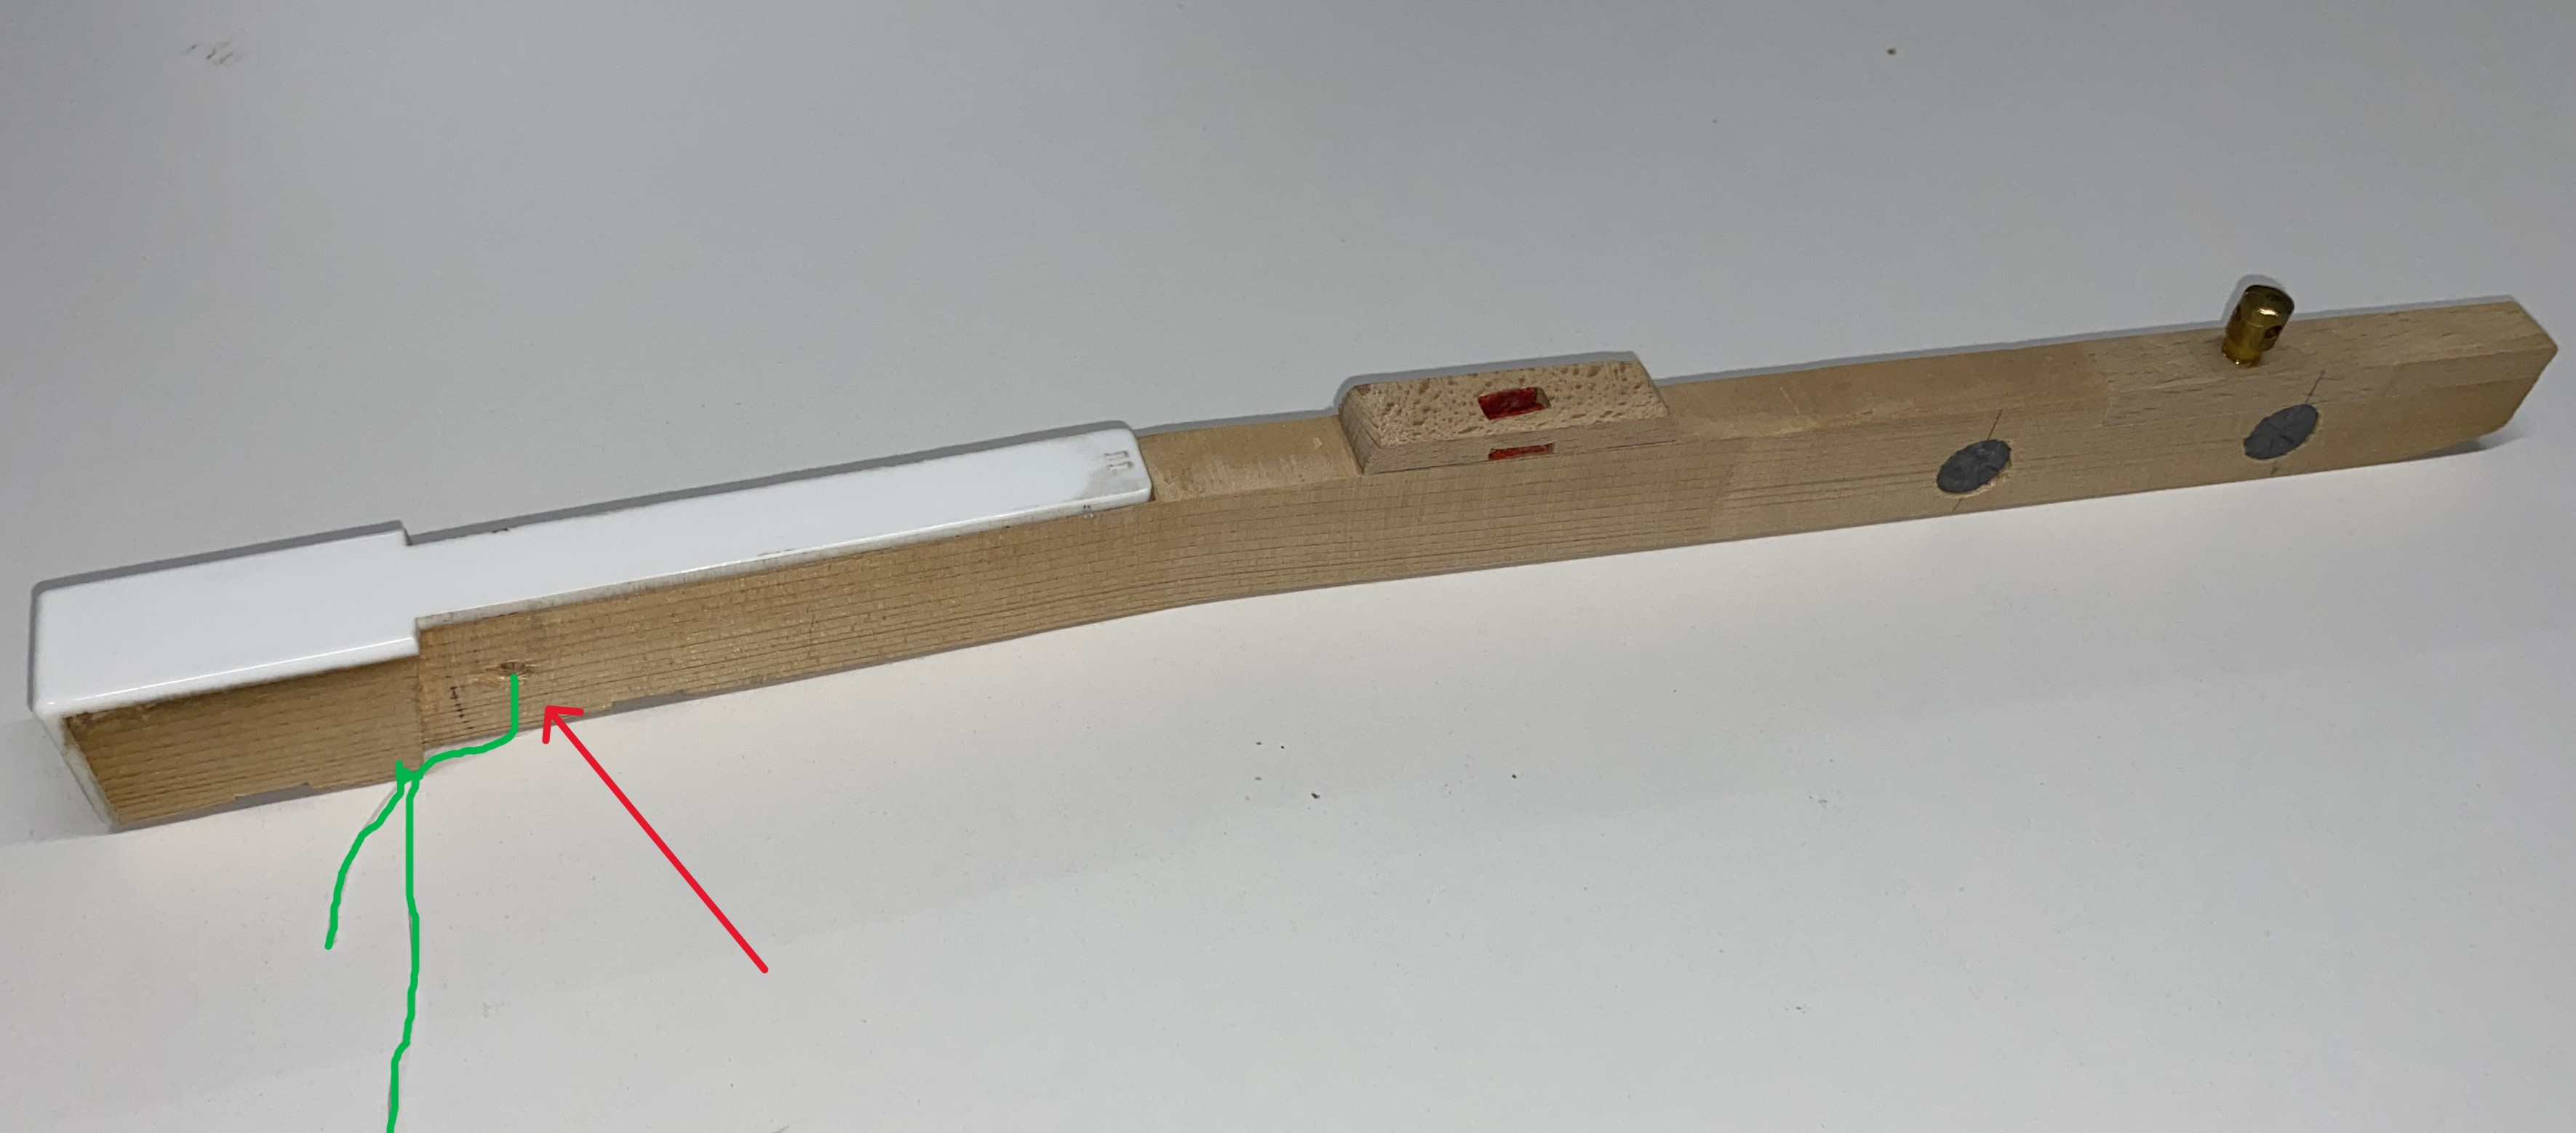
\includegraphics[width=8cm]{img/Taste_schraeg.jpg}
    \caption{Tastenbohrung}
    \label{img:Tastenbohrung}
\end{figure}


% @Note(Val): Der Satz ist mit den vielen Einschüben und Klammern schwer zu lesen. Lieber in 2 Sätze teilen und lesbarer machen
Anschließend wird jede Schnur jeweils durch ein senkrechtes Loch (rot in Abbildung \ref{fig:klaviatur} gekennzeichnet) im Klaviaturbalken (bzw. Tastenbrett), % @Note(Val): Nur einen Begriff einheitlich verwenden, sonst verwirrt es nur
worauf die Tasten liegen, in den Fußraum geführt.

\begin{figure}[htbp]
    \centering
    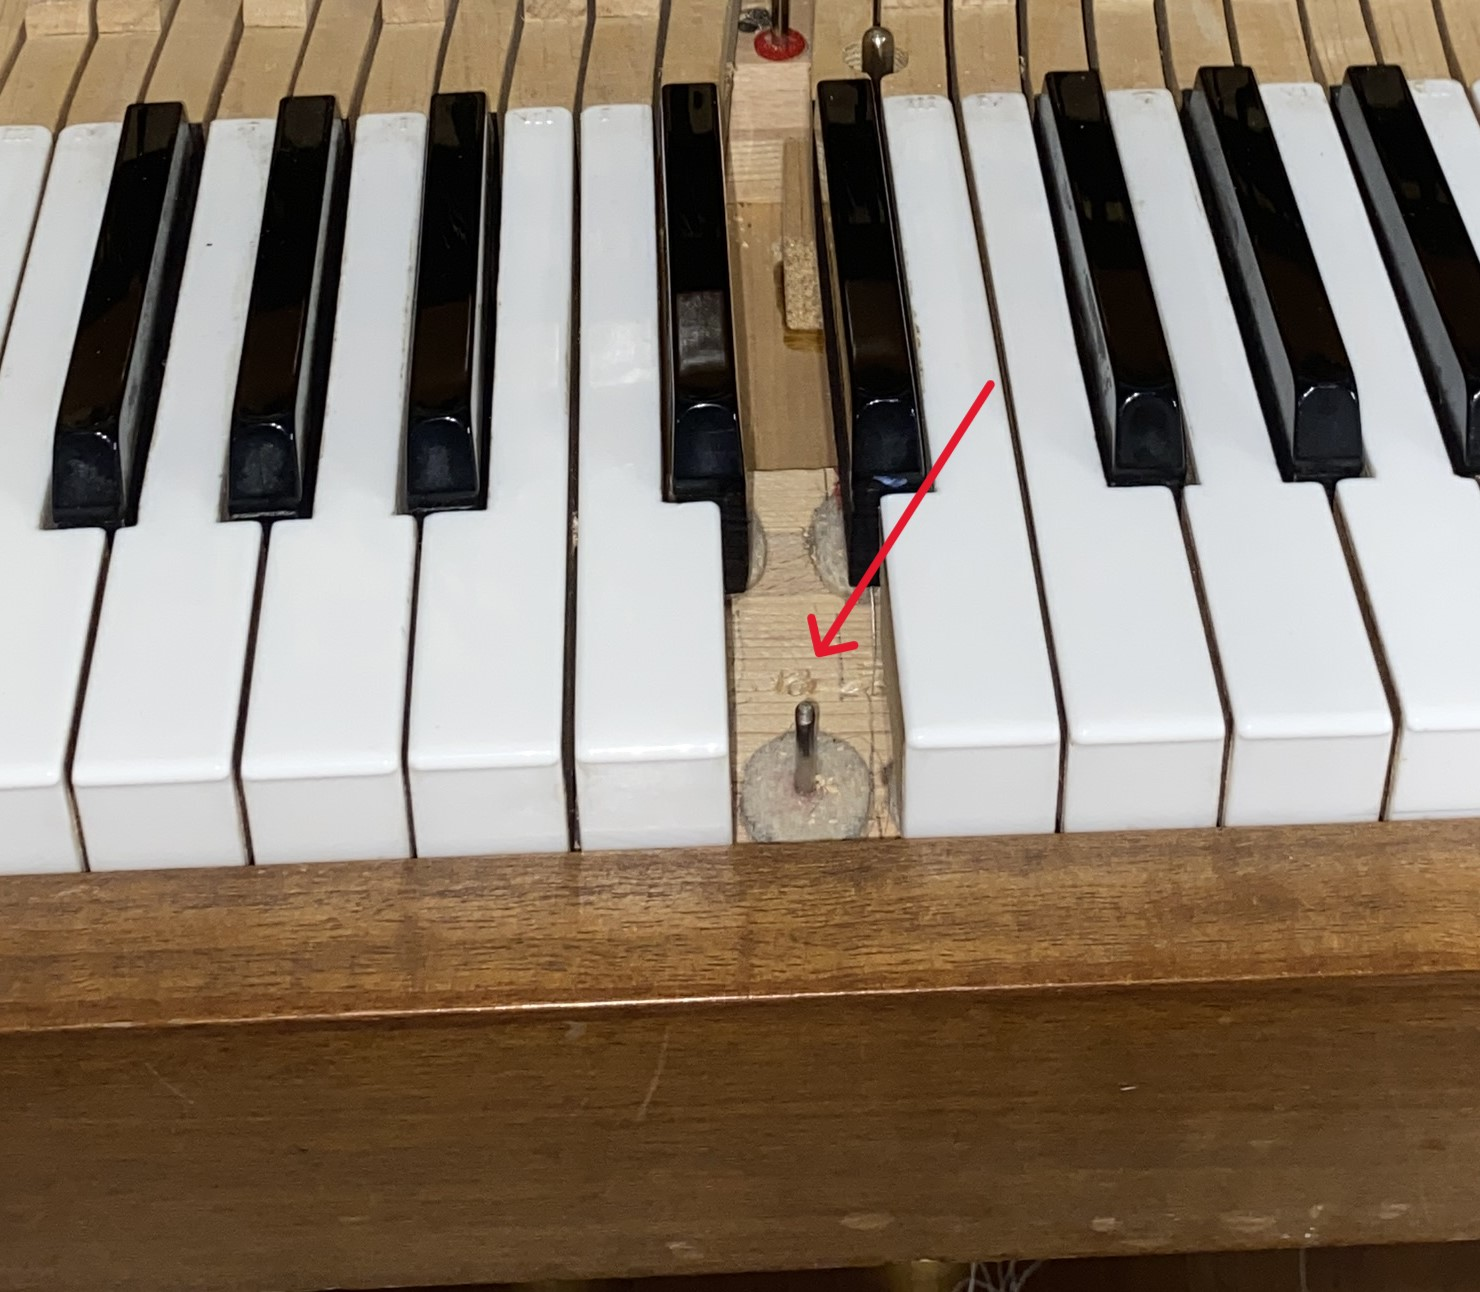
\includegraphics[width=5cm]{img/Klaviatur.jpg}
    \caption{Bohrung durch das Tastenbrett}
    \label{fig:klaviatur}
\end{figure}

\subsubsection{Anordnung der Aktuatoren}

Die Idee ist, die Hubmagnete parallel zur Klaviatur zu befestigen, um die Tasten möglichst senkrecht nach unten ziehen zu können.
Hierfür müssen folgende Aspekte berücksichtigt werden:

\begin{enumerate}
    \item Breite der Hubmagnete
    \item Hitzeentwicklung
    \item Seilführung
    \item Stabilität
    \item Modularität
\end{enumerate}

Ein Hubmagnet hat die Maße 2,5 cm x 6 cm.
Das Tastenbrett für 88 Tasten ist allerdings nur 140 cm breit, wodurch pro Tastenansteuerung nur ca. 1,6 cm zur Verfügung stehen.
Bildet man zwei Hubmagnetreihen übereinander, hat jede Tastenansteuerung 3,20 cm Platz.

Durch die 7mm Abstand ist eine Wärmeabfuhr über die Luft in geringem Ausmaß möglich.
Ob dies ausreicht, muss in späteren Tests (siehe Kapitel \ref{tests}) ermittelt werden.

Alle Seile werden pro Hubmagnetreihe, parallel zwischen Tasten und Hubmagneten verbunden.

Die Hubmagnete direkt unter dem Tastenbrett zu befestigen wäre eine triviale Lösung würde allerdings auf Kosten der Stabilität und Funkionalität gehen. % @Note(Val): Inwieweit? Hier fehlt eine Erklärung
Deshalb werden die Hubmagnete am Korpus des Klaviers (untere Frontplatte) befestigt.

Um die Austauschbarkeit der Komponenten zu verbessern, werden die Hubmagnete nicht direkt an der unteren Frontplatte,
sondern auf zwei Pressspanplatten (ca. 70 cm x 25 cm) befestigt, welche an vier Punkten mit dem Klavier verschraubt werden (siehe Abb. \ref{fig:BefestigungHubmagnete}). % @Note(Val): Die Abbildung zeigt mir nicht, wie die Platte mit dem Klavier verschraubt wird

\begin{figure}[htbp]
    \centering
    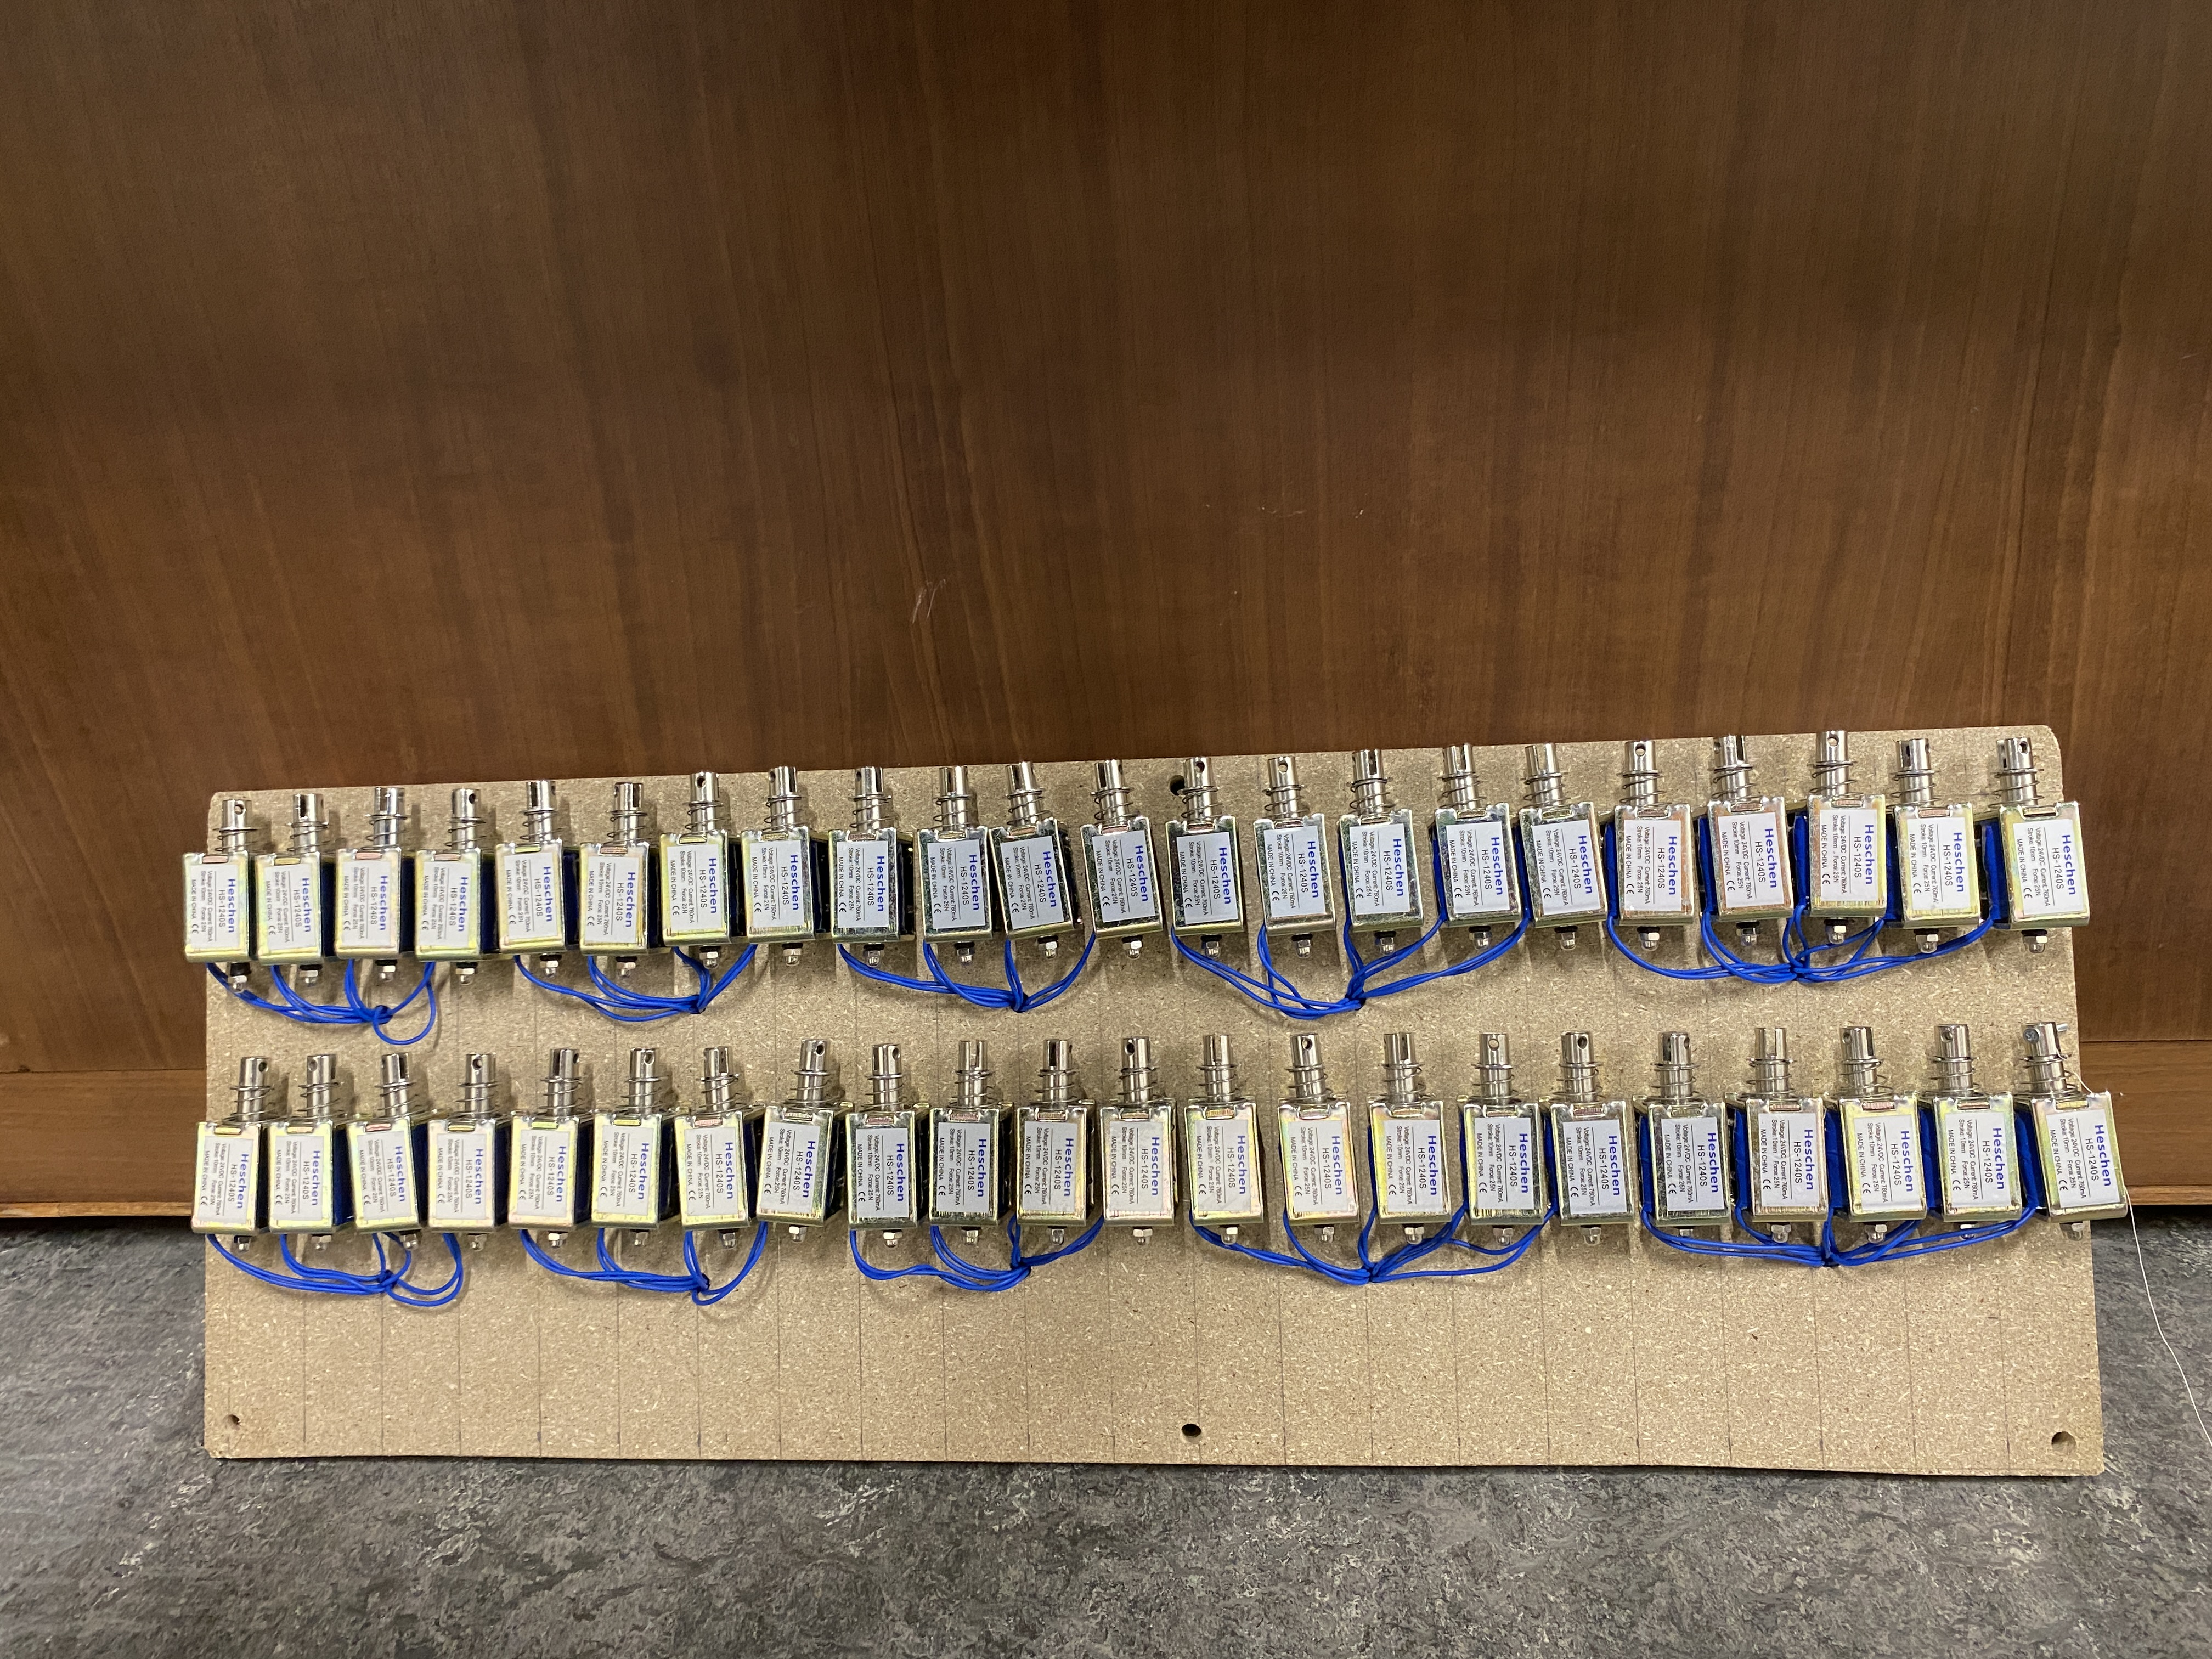
\includegraphics[width=5cm]{img/Magnetbrett.jpg}
    \caption{Befestigung der Hubmagnete}
    \label{fig:BefestigungHubmagnete}
\end{figure}

\subsubsection{Seilführung}

Würde man die Seile von den Tasten direkt zu den Hubmagneten führen,
hätte man deutliche Hub-Verluste und könnte unter Umständen die Tasten nicht mehr ausreichend stark betätigen, um einen Ton zu erzeugen.
\newline
In den folgenden Abbildungen ist die seitliche Ansicht des Klaviers gezeichnet.
Dabei repräsentieren der schwarze bzw. weiße Block jeweils eine schwarze bzw. weiße Taste.
Der grüne und pinke Strich stehen für die Seile, die den Hubmagneten mit dem Loch in der Taste verbinden.
Unten links sind die zwei übereinanderliegenden Solenoid-Reihen in blau abgebildet.
Der schwarze Strich repräsentiert den Stab im Hubmagneten. % @Note(Val): Die Farbe vom Solenoid kannst du dir fast sparen, wenn du die Grafik so klein abbildest. Das blau kann ich nur mit viel reinzoomen sehen
\newline
Abbildung \ref{img:Umlenkung_locker} zeigt den intuitiven Aufbau mit ausgeschaltetem Solenoid und entsprechend entspanntem Seil und.
Abbildung \ref{img:Umlenkung_gezogen} zeigt den selben Aufbau mit dem Unterschied, dass der Solenoid hier angezogen ist.

\begin{figure}[htbp]
    \centering
    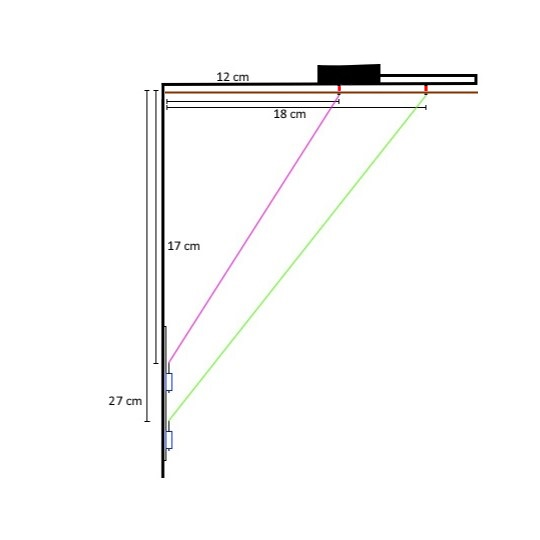
\includegraphics[width=6cm, height=8cm]{img/Umlenkung_locker}
    \caption{Taste locker ohne Umlenkung}
    \label{img:Umlenkung_locker}
\end{figure}

% @Note(Val): Es wäre besser, wenn sich die beiden Bilder mehr unterscheiden würden. Falls das erste Bild stärker zeigen könnte, dass die Seile locker sind oder es eine Kennzeichnung bei den Seilen gibt, wäre das gut. Alternativ könnten auch die Tasten runtergedrückt sein, um anzuzeigen, dass diese damit betätigt werden
\begin{figure}[htbp]
    \centering
    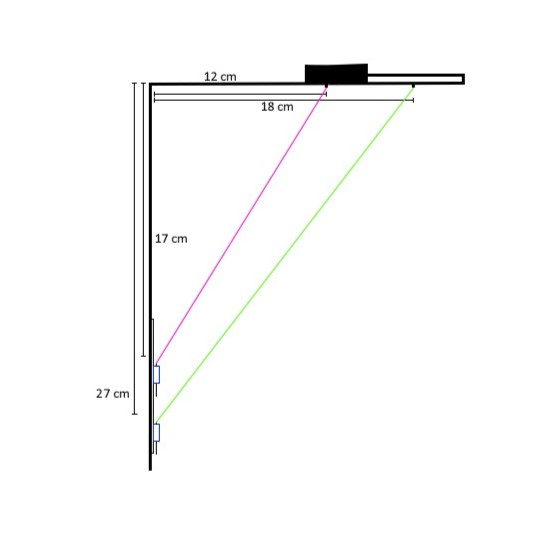
\includegraphics[width=6cm, height=8cm]{img/Umlenkung_gezogen}
    \caption{Taste gezogen ohne Umlenkung}
    \label{img:Umlenkung_gezogen}
\end{figure}

% @Note(Val): Warum gibt es hier einen forcierten Seitenumbruch? Braucht es das?
\newpage

Mit diesem intuitiven Aufbau funktioniert das Betätigen der Tasten nicht, da diese nicht weit genug heruntergezogen werden.
Um den gesamten Hub des Magneten zu Nutzen und an die Taste weiterzugeben, müssen Umlenkungen eingebaut werden.
Mittels dieser Umlenkung, die mit einem PVC-Rohr umgesetzt werden kann, werden die Seile so geführt, das sie senkrecht auf die Hubmagnete fallen.
Somit wird die Tiefe, mit der die Tasten gedrückt werden, wieder auf annähernd 1 cm erhöht, was dem Hub des Magneten entspricht..

% @Note(Val): Wenn die Umlenkung weiter unten im Bild wäre, wären die unterschiedlichen Linien leichter zu sehen
\begin{figure}[htbp]
    \centering
    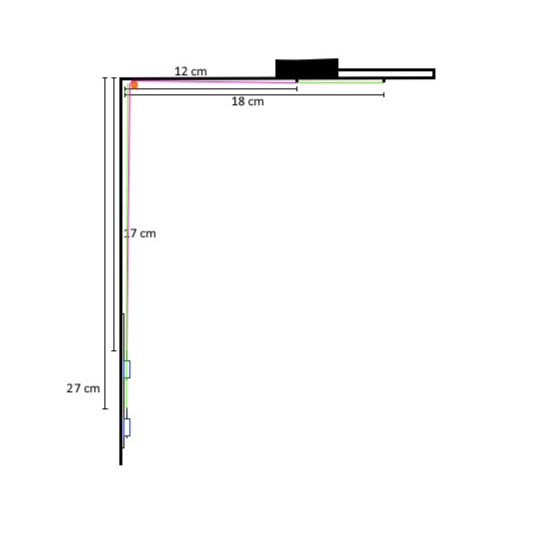
\includegraphics[width=6cm, height=8cm]{img/mitUmlenkung_locker}
    \caption{Taste mit Umlenkung}
\end{figure}


% @Note(Val): Entweder machst du das hier als Bullet-Points or mit vollständigen Sätzen. Aber so ist das ein bisschen merkwürdig
Dies kann auch mathematisch bewiesen werden:
\newline geg.: % @Note(Val): "gegeben" aber ohne "gesucht" und ohne Demarkierung wann etwas nicht mehr gegeben ist... können wir das "geg." einfach streichen?
\newline Strecke bis zur ersten Reihe Hubmagnete h1 = 17 cm % @Note(Val): Strecke von wo?
\newline Strecke bis zur zweiten Reihe Hubmagnete h2 = 27 cm
\newline Strecke bis zu den schwarzen Tasten t1 = 12 cm
\newline Strecke bis zu den weißen Tasten t2 = 18 cm
\newline Seil zur schwarzen Taste im entspannten Zustand $ht1_{entspannt}$ % @Note(Val): Du meinst Seillänge? Ist die Seillänge nicht konstant? Warum berechnen wir die?
\newline Seil zu den weißen Tasten im entspannten Zustand $ht2_{entspannt}$
\newline $ht1_{entspannt}$ = $\sqrt {h1^{2} + t1^{2}}$ = 20.81 cm
\newline $ht2_{entspannt}$ = $\sqrt {h2^{2} + t2^{2}}$ = 32.45 cm
\newline $ht1_{gespannt}$ = $\sqrt {(h1 + 1) ^{2} + t1^{2}}$ = 21.63 cm
\newline $ht2_{gespannt}$ = $\sqrt {(h2 + 1)^{2} + t2^{2}}$ = 33.29 cm

Die Differenz zwischen $ht1_{gespannt}$ und $ht1_{entspannt}$ (bzw. ht2) beschreibt die Tiefe, die eine Taste gedrückt werden kann.
\newline Diese beträgt also ohne Optimierung nur 0.82 cm, bzw. 0.84 cm. % @Note(Val): "ohne Optimierung" - was für Optimierungen wären hier denn überhaupt möglich? Ist die Verwendung einer Umlenkun nicht schon eine Optimierung?

Um also die Intensität des Tastendrucks besser steuern zu können und um die Haltbarkeit des Materials zu verlängern,
sollte die Reibung am Seil möglichst gering gehalten werden.
Dazu können mittels Rohren, welche waagerecht unter dem Klaviaturbalken entlang der Löcher montiert werden können (siehe Abbildung \ref{fig:fussraum}), die Seile umgelenkt und
entlang der Verkleidung zur unteren Frontplatte des Klaviers geführt werden.
Das hat den positiven Nebeneffekt, dass die Pianist:innen nicht durch Platzmangel im Beinbereich eingeschränkt sind.


\begin{figure}[htbp]
    \centering
    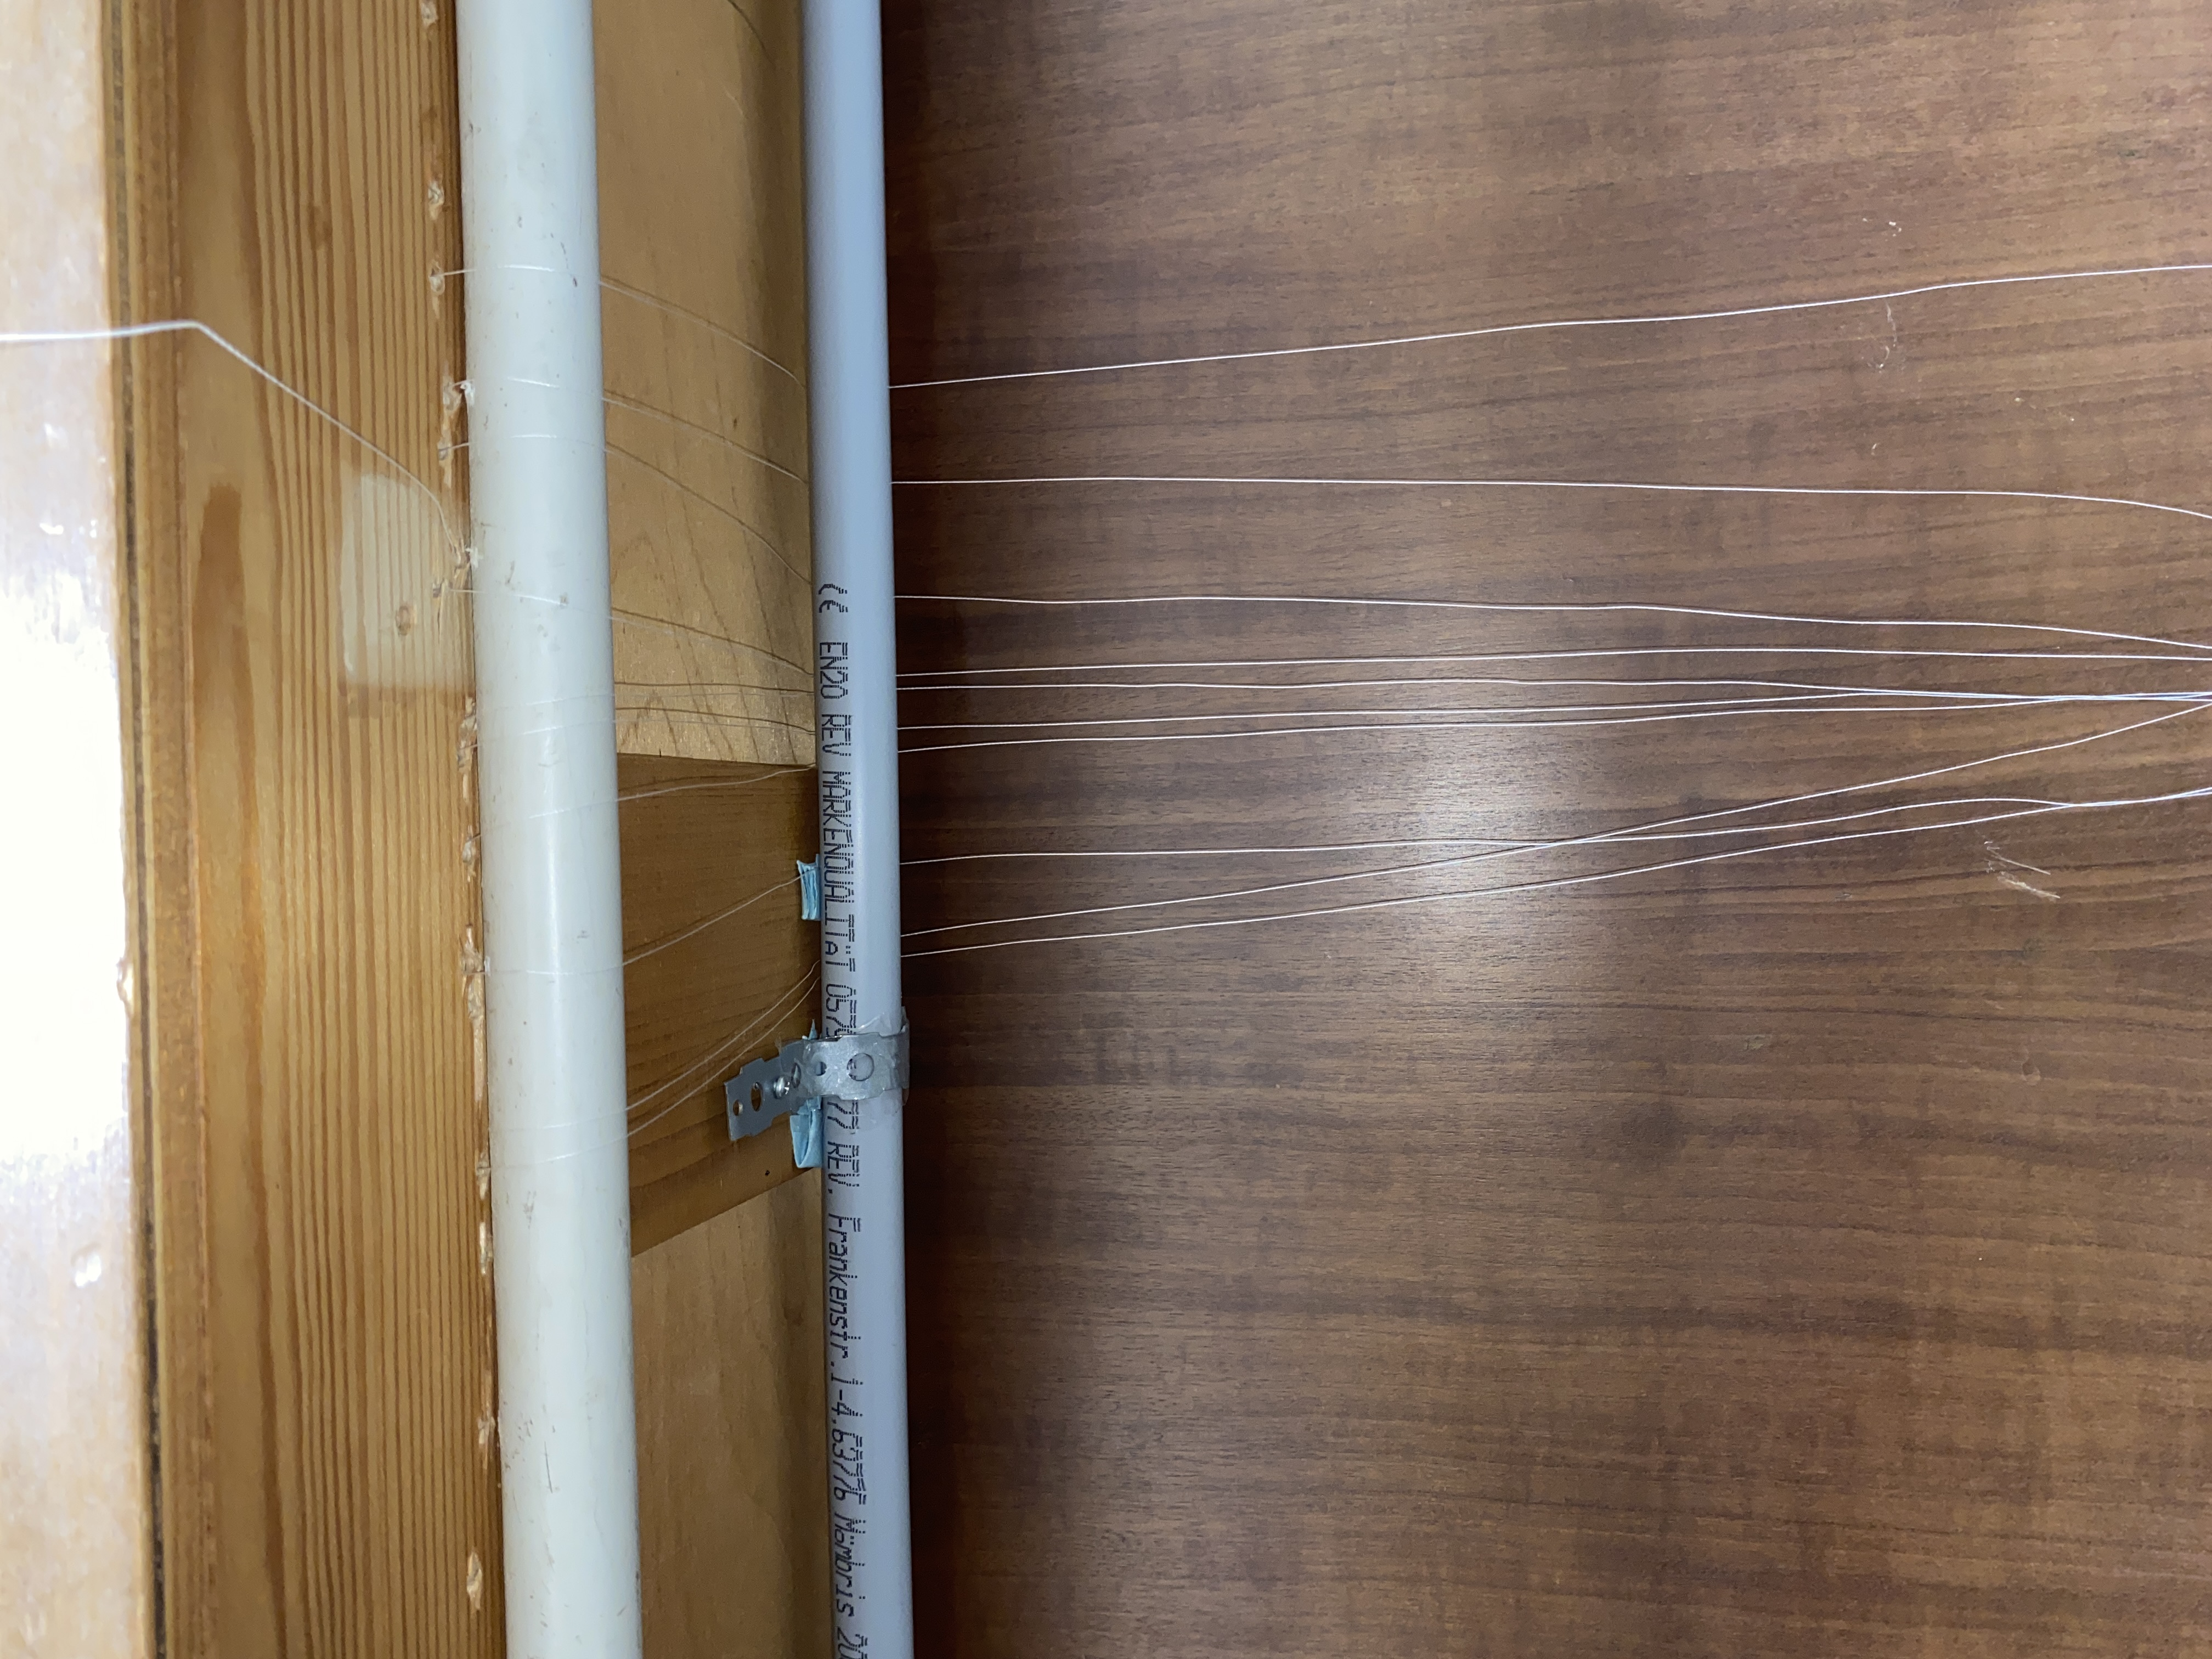
\includegraphics[width=5cm,angle=-90]{img/Fussraum.jpg}
    \caption{Fußraum des Klaviers}
    \label{fig:fussraum}
\end{figure}


\subsubsection{Auswahl des Seils}

Wie eben beschrieben wird das Ziehen durch ein Seil ermöglicht.
Dafür wird ein leichtes, formbares, unelastisches und dehnungsresistentes Material benötigt, welches die Hubmagnete mit den Tasten verbindet.
Je leichter das Material ist, desto weniger geht die Genauigkeit der Kraftübertragung zwischen den Magneten und den Tasten verloren.
Durch die Formbarkeit kann der Knoten sehr eng an der Taste geschnürt werden, wodurch das Ansprechverhalten schneller erfolgen kann.
Da die Anschläge ruckartige Bewegungen sind, ist es wichtig ein unelastisches Seil zu verwenden.
Um häufiges Nachspannen oder Austauschen des Seils entgegenzuwirken, sollte dies so dehnungsresistent wie möglich sein.

% @Note(Val): Ab hier wird in der Vergangenheit gesprochen. Ich nehme an, dass das hier aber ok ist, da davon gesprochen wird, was umgesetzt und getestet wurde.
\paragraph{Nähgarn}

Als Erstes wurde Nähgarn, welches zur Hand war, getestet.
Auch doppelt verlegt hielt es der ruckartigen Ziehbewegung (mit 25N) des Hubmagnetens nicht stand.
Vier Fäden funktionierten zu Beginn gut, leierten allerdings schnell aus.

\paragraph{Nylonsaiten}

Als Nächstes wurde die g-Saite einer Gitarre verwendet.
Durch den höheren Durchmesser und das stärkere Material riss und leierte die Saite nicht aus.
Da die Saite kaum Flexibilität liefert, war die Befestigung an der Taste jedoch äußerst schwierig.
Beim Ziehen des Magnetens wurde erst die lockere Schlaufe an der Taste gestreckt, wodurch nicht der vollständige Hub des Magnetens auf die Taste übertragen wurde.

\paragraph{Angelschnur}

% @Note(Val) "Aus Erfahrungen [...] konnte eine Schnur gefunden werden" klingt sehr falsch
Aus Erfahrungen aus dem Angelbereich konnte schnell eine geeignetere Schnur gefunden werden.
Genauer handelt es sich um eine geflochtene Schnur aus Polyethylene.
Mit einem Durchmesser von 1.6 mm ist sie nicht nur sehr dünn und flexibel, sondern kann auch bis zu 7 kg standhalten.
Nach ausgiebigem Testen ist eindeutig, dass die Angelschnur die Anforderungen erfüllt.
Damit ist nun auch das Spielen des Forellenquintetts von Schubert ein Leichtes.

\subsection{Klangdämpfung der Aktuatoren}

\chapterauthor{Olivier Stenzel}

Die Hubmagnete machen beim Anschlagen laute \enquote{Klack} Geräusche, welche von der Melodie des Klaviers ablenken.
Genauer handelt es sich um den Metall-Anker, der gegen das Ende des Metall-Gehäuses stößt.
Auch hierfür gab es mehrere Ideen und Tests, um das Geräusch zu dämpfen:

\subsubsection{Isolierfolie}

Die erste Überlegung war die Auskleidung des Innenraums der Hubmagnete mit Isolierfolie.
Diese Idee wurde wieder verworfen, da das Wissen über die Hitzeentwicklung zu diesem Zeitpunkt noch zu gering war, um sicherzustellen, dass die Isolierung dem standhält. % "dem" meint die Hitzeentwicklung? Dann müsste es "ihr" sein.

\subsubsection{Gummi-Stopper}

Die nächste Idee war das Limitieren des Schlags durch Gummiringe (Dichtungsringe) % @Note(Val): Ein Wort verwenden, oder in einen Satz einbringen (z.B. "Dichtungsringe aus Gummi" oder so)
zwischen Anker und dem äußeren Gehäuse.
Da für die Befestigung keine zufriedenstellende Lösung gefunden wurde, wurde auch diese Idee verworfen.
zurück schellen zu hoch, als dass wir die Klangdämpfung umsetzen würden. % @Note(Val): Das ist kein richtiger Satz und ich habe keine Ahnung was du damit aussagen wolltest. Satz streichen oder verbessern

\subsubsection{Schaumstoff}

Wie im Abbildung \ref{fig:schaumstoff} zu sehen ist, wurde die \enquote{Gummi-Stopper}-Idee durch den Einsatz von Schaumstoff leicht modifiziert. \newline
+ Klopfgeräusch wird vollständig verhindert \newline
- Durch den Schaumstoff wird 1mm des Hubs nicht verwendet, weshalb nur noch 9mm übrig bleiben \newline
- Der Aufbau ist optisch nicht besonders ansprechend

\begin{figure}[htbp]
    \centering
    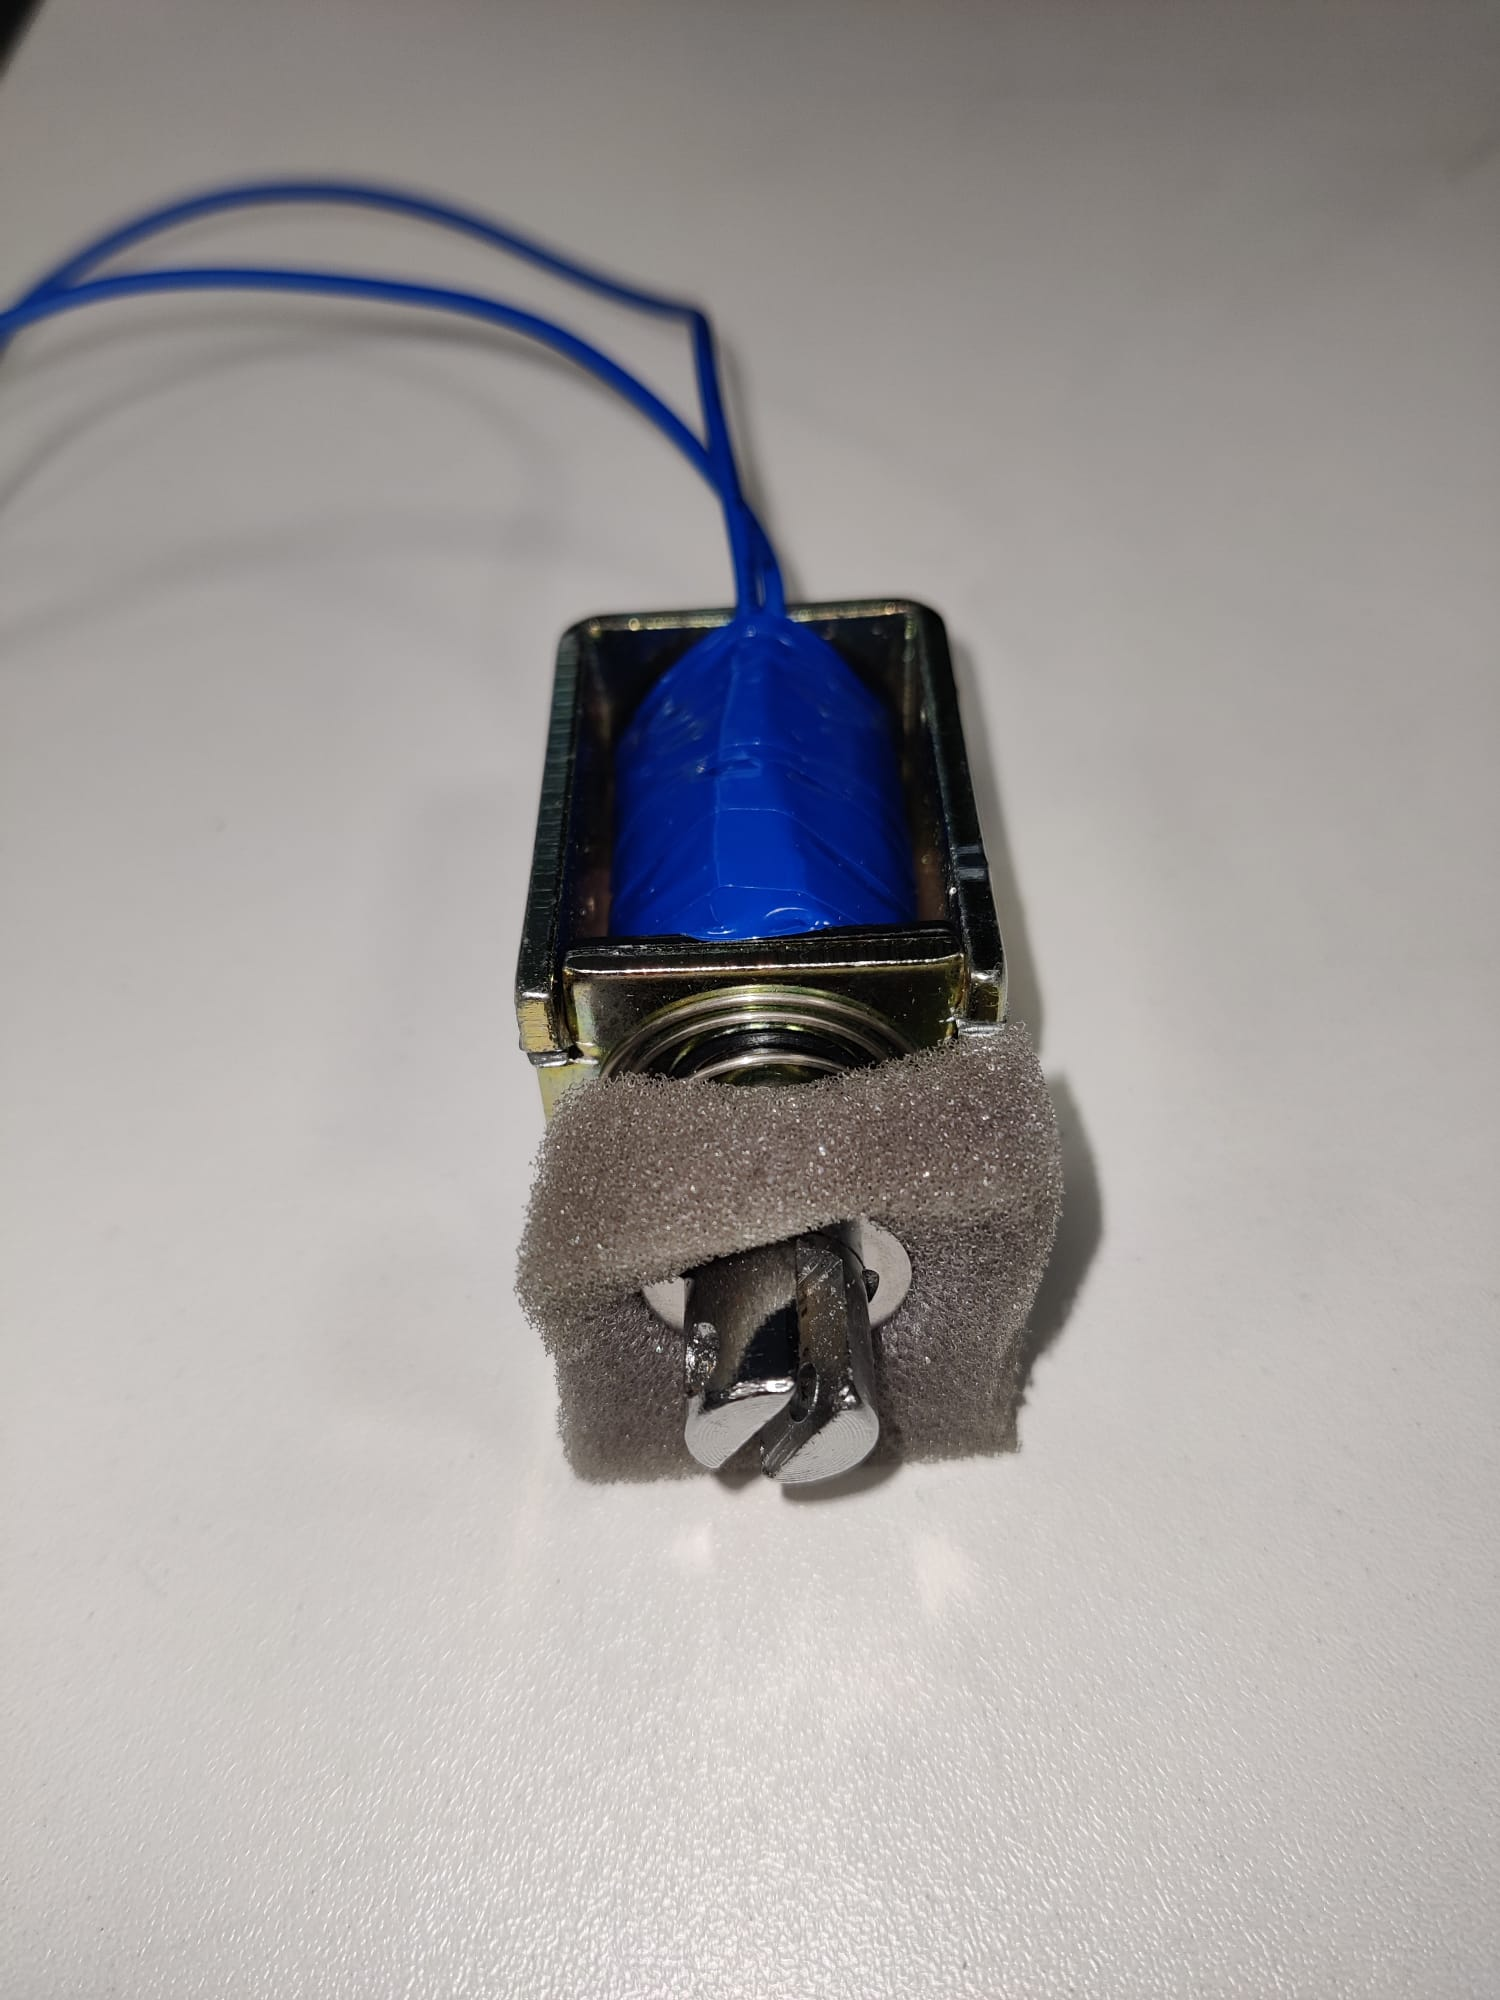
\includegraphics [width=4cm] {img/Daempfung_Schaumstoff}
    \caption{Hubmagnet: Dämpfung mit Schaumstoff}
    \label{fig:schaumstoff}
\end{figure}

\paragraph{Seil (2mm Durchmesser) um den Anker}

Um das \enquote{Problem} der schlechten Ästetik beim Schaumstoff zu beseitigen, wird nun ein 2mm dickes Seil im Inneren des Gehäuses um den Anker gewickelt. \newline
+ Auch hier konnte das Klopfen vollständig beseitigt werden \newline
+ Von außen sieht man keine Veränderung \newline
+ Das Seil scheint ausführlichen Tests nach der Hitzeentwicklung gut Stand zu halten  \newline
- Durch die Dicke des Seils, werden 2mm des Hubs nicht verwendet, weshalb nur noch 8mm übrig bleiben.

\begin{figure}[htbp]
    \centering
    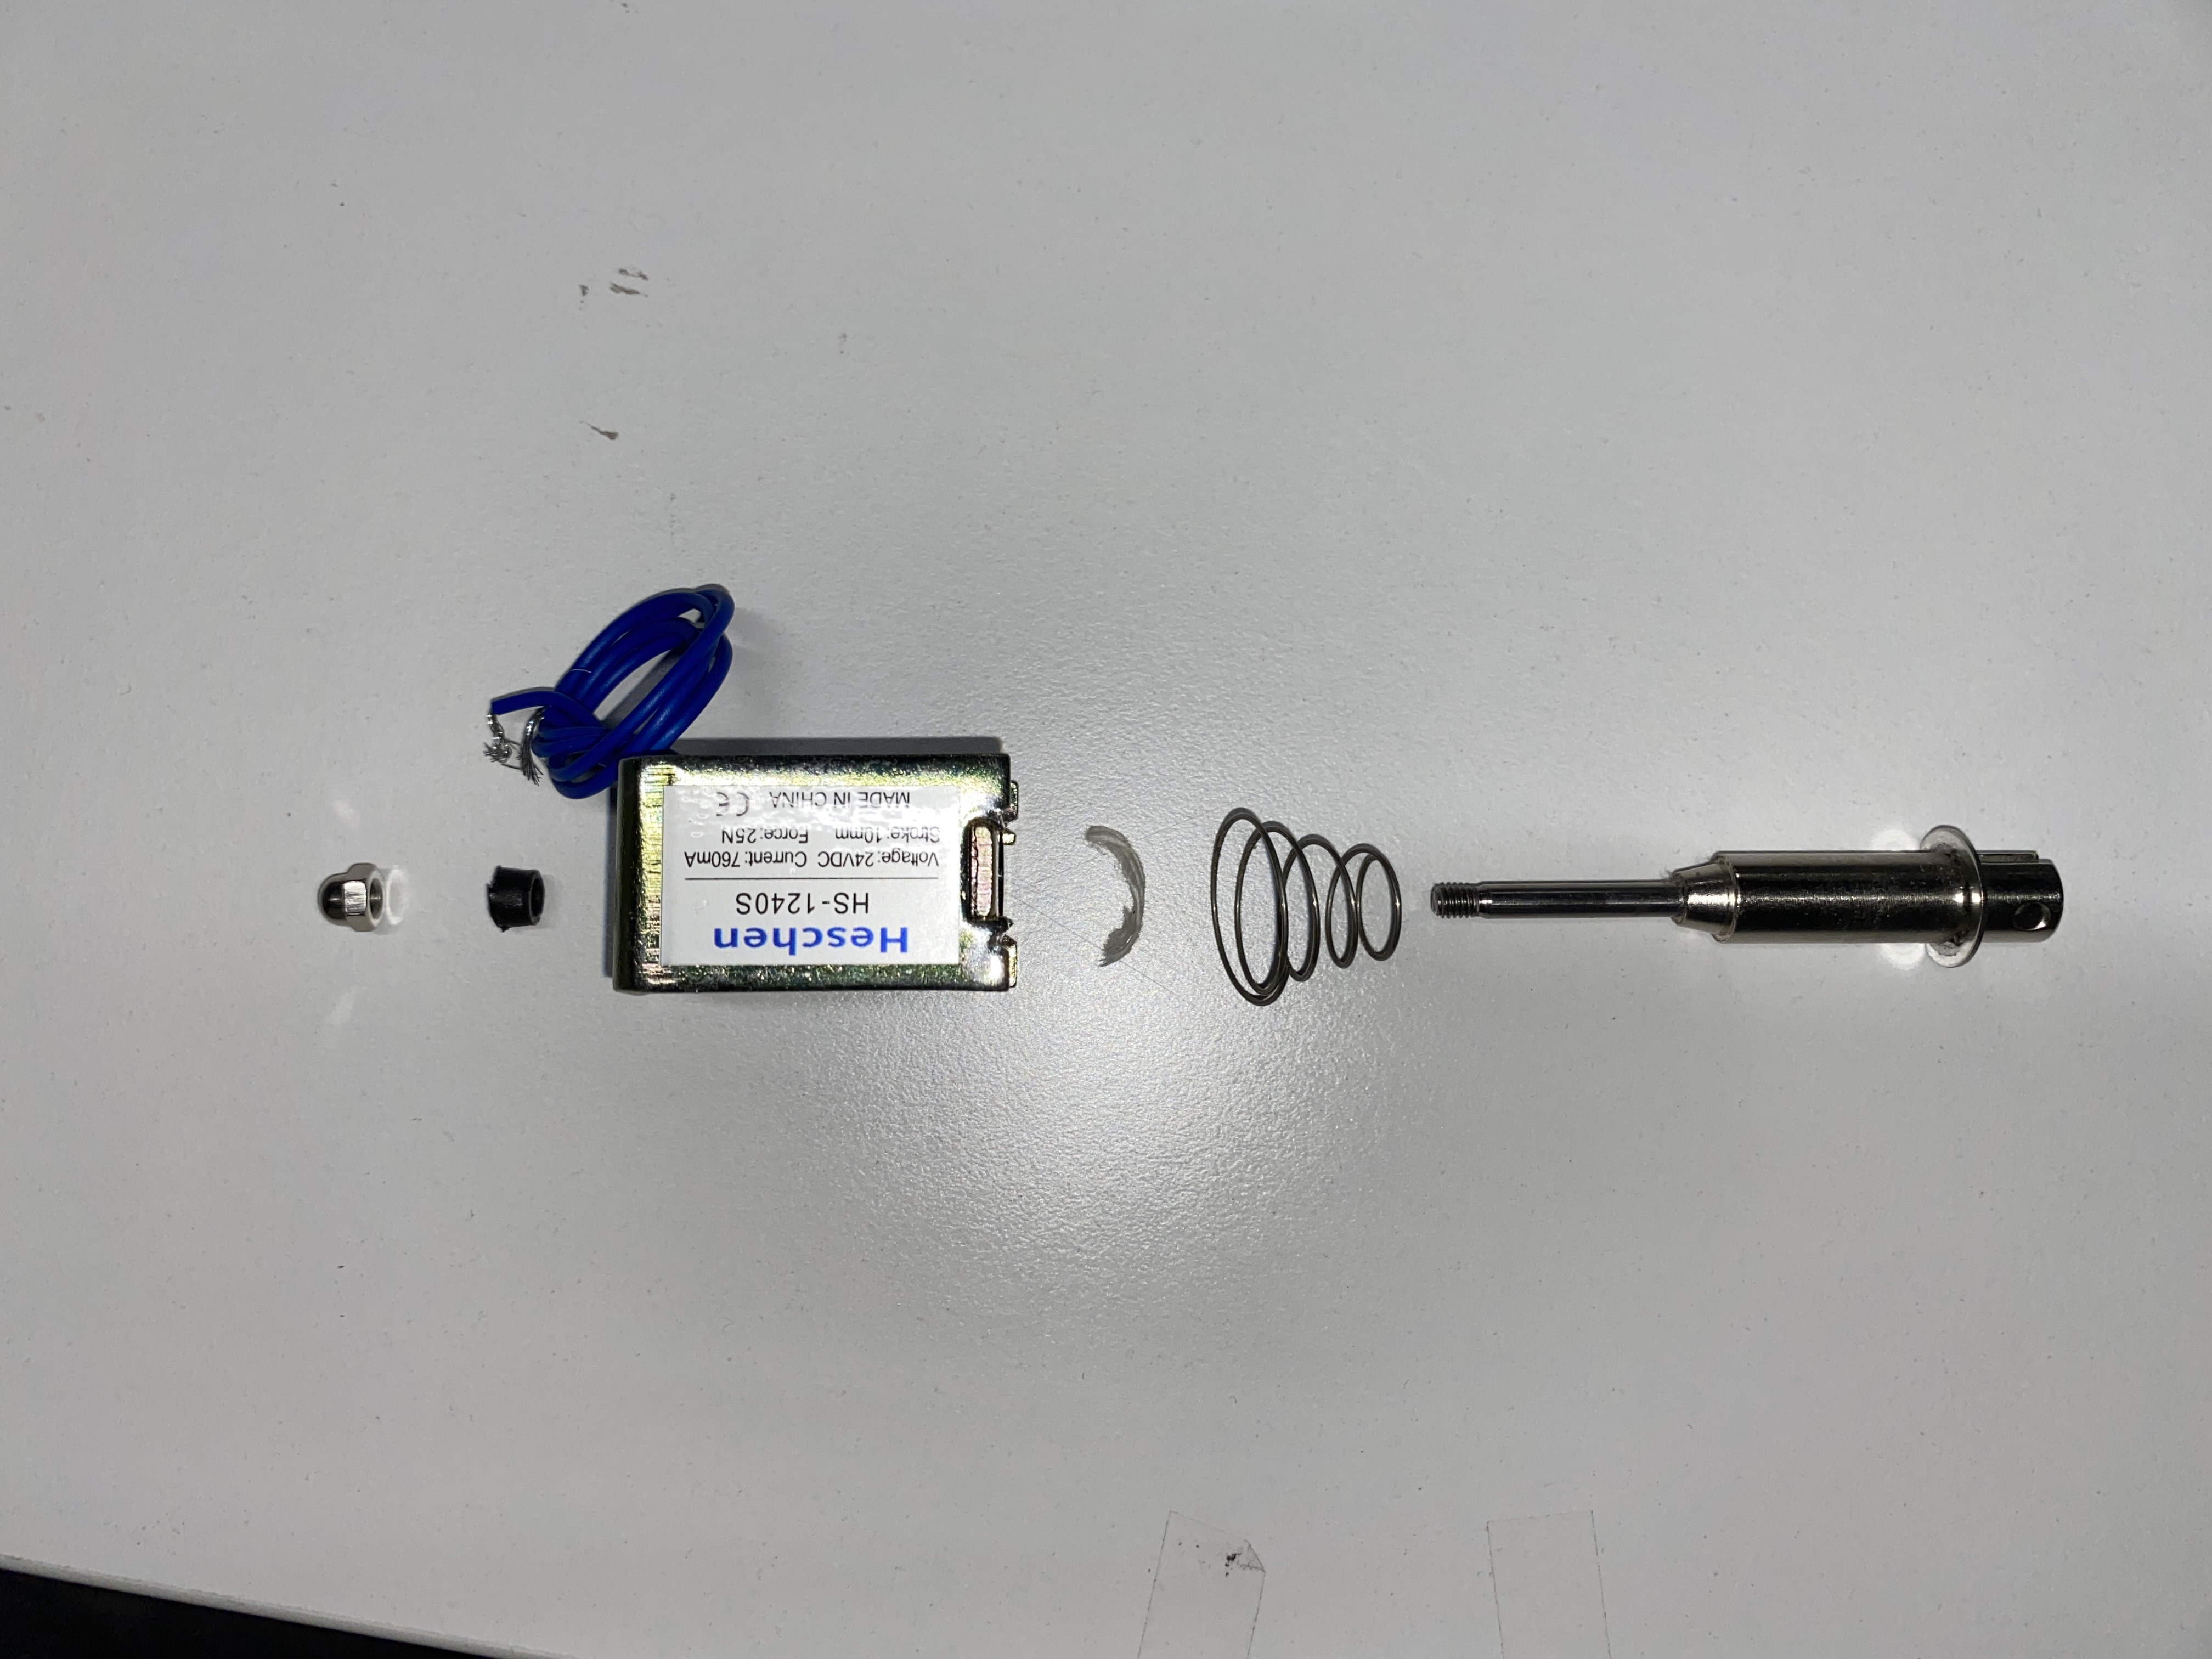
\includegraphics [width=4cm] {img/Hubmagnet_Seil_Daempfung.jpg}
    \caption{Hubmagnet: Dämpfung mit Seil}
\end{figure}


\subsection{Klavieranbau}
Im Rahmen des Protoypen wurde die Elektrik nicht fest am Klavier verschraubt.
Das Brett mit den Hubmagneten wurde stattdessen nur an das Klavier angelehnt, während die Angelschnüre die Verbindung zu den Tasten herstellen.
Gespannt werden die Seile durch eine Schrauben-Mutter Konstruktion (siehe Abschnitt \ref{subsec:VerbindungTastenAktuatoren}).

\subsection{Ergebnisse des Prototypen}
% @TODO(Val):
Das Anspielen klappt iwie aber noch hakelig.
% TODO(Jay): was funktioniert genau, was ist noch einfach hinzuzufügen, wo gabs Probleme


